\documentclass[10pt, draftclsnofoot, onecolumn]{IEEEtran}
  \usepackage{graphicx}
  \usepackage{url}
  \usepackage{setspace}
  
  \usepackage[margin=0.75in]{geometry}
  \usepackage{geometry}
  \usepackage{hyperref}
  \usepackage{caption} 
  \usepackage{float}
  \usepackage{rotating} 
  \usepackage{ragged2e} % provides \RaggedLeft
  \hypersetup{
      colorlinks,
      citecolor=black,
      filecolor=black,
      linkcolor=black,
      urlcolor=black
  }
  \geometry{textheight=9.5in, textwidth=7in}
  
  % 1. Fill in these details
  \def \CapstoneTeamName{		The Dream Team}
  \def \CapstoneTeamNumber{		57}
  \def \GroupMemberOne{			Daniel Schroeder}
  \def \GroupMemberTwo{			Aubrey Thenell}
  \def \GroupMemberThree{			Parker Bruni}
  \def \CapstoneProjectName{		A Scalable Web Application Framework for Monitoring Energy Usage on Campus  }
  \def \CapstoneSponsorCompany{	Oregon State Office of Sustainability}
  \def \CapstoneSponsorPerson{		Jack Woods}
  
  % 2. Uncomment the appropriate line below so that the document type works
  \def \DocType{		%Problem Statement
          %Requirements Document
          %Technology Review
          Design Document
          %Progress Report
          }
        
  \newcommand{\NameSigPair}[1]{\par
  \makebox[2.75in][r]{#1} \hfil 	\makebox[3.25in]{\makebox[2.25in]{\hrulefill} \hfill		\makebox[.75in]{\hrulefill}}
  \par\vspace{-12pt} \textit{\tiny\noindent
  \makebox[2.75in]{} \hfil		\makebox[3.25in]{\makebox[2.25in][r]{Signature} \hfill	\makebox[.75in][r]{Date}}}}
  % 3. If the document is not to be signed, uncomment the RENEWcommand below
  %\renewcommand{\NameSigPair}[1]{#1}
  
  %%%%%%%%%%%%%%%%%%%%%%%%%%%%%%%%%%%%%%%
  \title{CS 450 Computer Graphics: \linebreak Final Project}
  \author{Daniel Schroeder}
  \date{\today}
  
  \begin{document}
  \maketitle
  \vspace{2cm}
  \begin{center}
  \noindent \textbf{Abstract} \\
              \indent This document is a report outlining my final implementation of my CS 450 Computer Graphics final project. This report details how I coded my program, how my final implementation is different from my proposal, and notable displays of OpenGL expertise!
  \end{center}         
  
  \newpage
  \pagenumbering{arabic}
  \tableofcontents
  \newpage

\section{What you actually did for your project, with images}
\subsection{Building Shaders}
\begin{center} 
  \begin{figure}[H]
      \centering
      \includegraphics[width=8cm,height=8cm]{skyview.eps}
  \end{figure}
\end{center}  
\subsection{Grass Shaders}
\begin{center} 
  \begin{figure}[H]
      \centering
      \includegraphics[width=8cm,height=8cm]{grass.eps}
  \end{figure}
\end{center}  
\subsection{Road Texture Mapping}
\begin{center} 
  \begin{figure}[H]
      \centering
      \includegraphics[width=8cm,height=8cm]{street.eps}
  \end{figure}
\end{center}  
\subsection{Skydome Shader}
\begin{center} 
  \begin{figure}[H]
      \centering
      \includegraphics[width=8cm,height=8cm]{skydome.eps}
  \end{figure}
\end{center}  
\section{How your project differs from what you proposed, and why}
\section{Any impressive cleverness you want us to know about}
\section{What you learned from doing this project (i.e., what you know now that you didn't know when you started)}
\section{Any images that are especially representative of what you did}
\section{A link to the video showing off your project.}
\newpage
\section{Proposal}
\noindent\textbf{Daniel Schroeder}\\
\textbf{schrodan@oregonstate.edu}\\
\textbf{Final Project Proposal}\\
\vspace{1.5cm}

For my final project, I would like to create a city-scape where the user can ``move'' around and traverse the streets. Similar to the video we saw flying over Chicago, I would like to create a scene with buildings of different shapes and sizes but with the eye positing at ground level. This program will involve shaders for coloring the buildings, geometric modeling for generating the buildings, and more versatile use of gluLookAt and eye position techniques to allow the user to ``move'' and ``look'' around.
I think this project should be worth 200 points because it combines a lot of different aspects from previous programs and applies the different techniques to multiple objects (buildings) in order to create a large scene. I've included a crude image of what the city-scape might look like.

\vspace{1.5cm}
\begin{center} 
\begin{figure}[H]
    \centering
    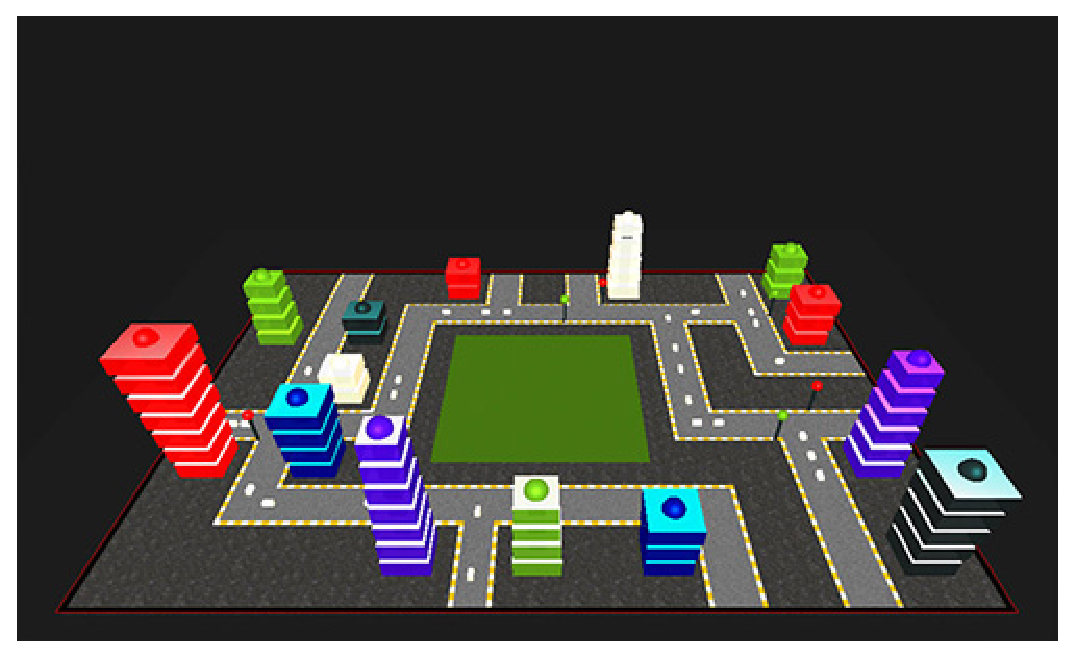
\includegraphics[width=8cm,height=8cm]{city.eps}
\end{figure}
\end{center}
\end{document}
